\section{Đánh giá hiệu năng và độ trễ}
Hiệu năng và độ trễ là tiêu chí trọng tâm của hệ thống phân giải tên miền (DNS Resolver), nhất là khi kết hợp chấm điểm ngữ vựng và đối chiếu tình báo mối đe dọa. Việc đánh giá Safe Zone được thực hiện bằng công cụ giả lập tải trong môi trường độc lập để đảm bảo khách quan.

\subsection{Đánh giá độ trễ phân giải (Latency)}

Thử nghiệm đo lường thời gian đáp ứng của hệ thống qua 3 kịch bản: truy vấn từ bộ nhớ đệm RAM (Redis Cache Hit), từ cơ sở dữ liệu cục bộ (SQLite Local Hit), và truy vấn mới cần phân tích ngữ vựng cục bộ (Cache Miss).

\begin{figure}[H]
    \centering
    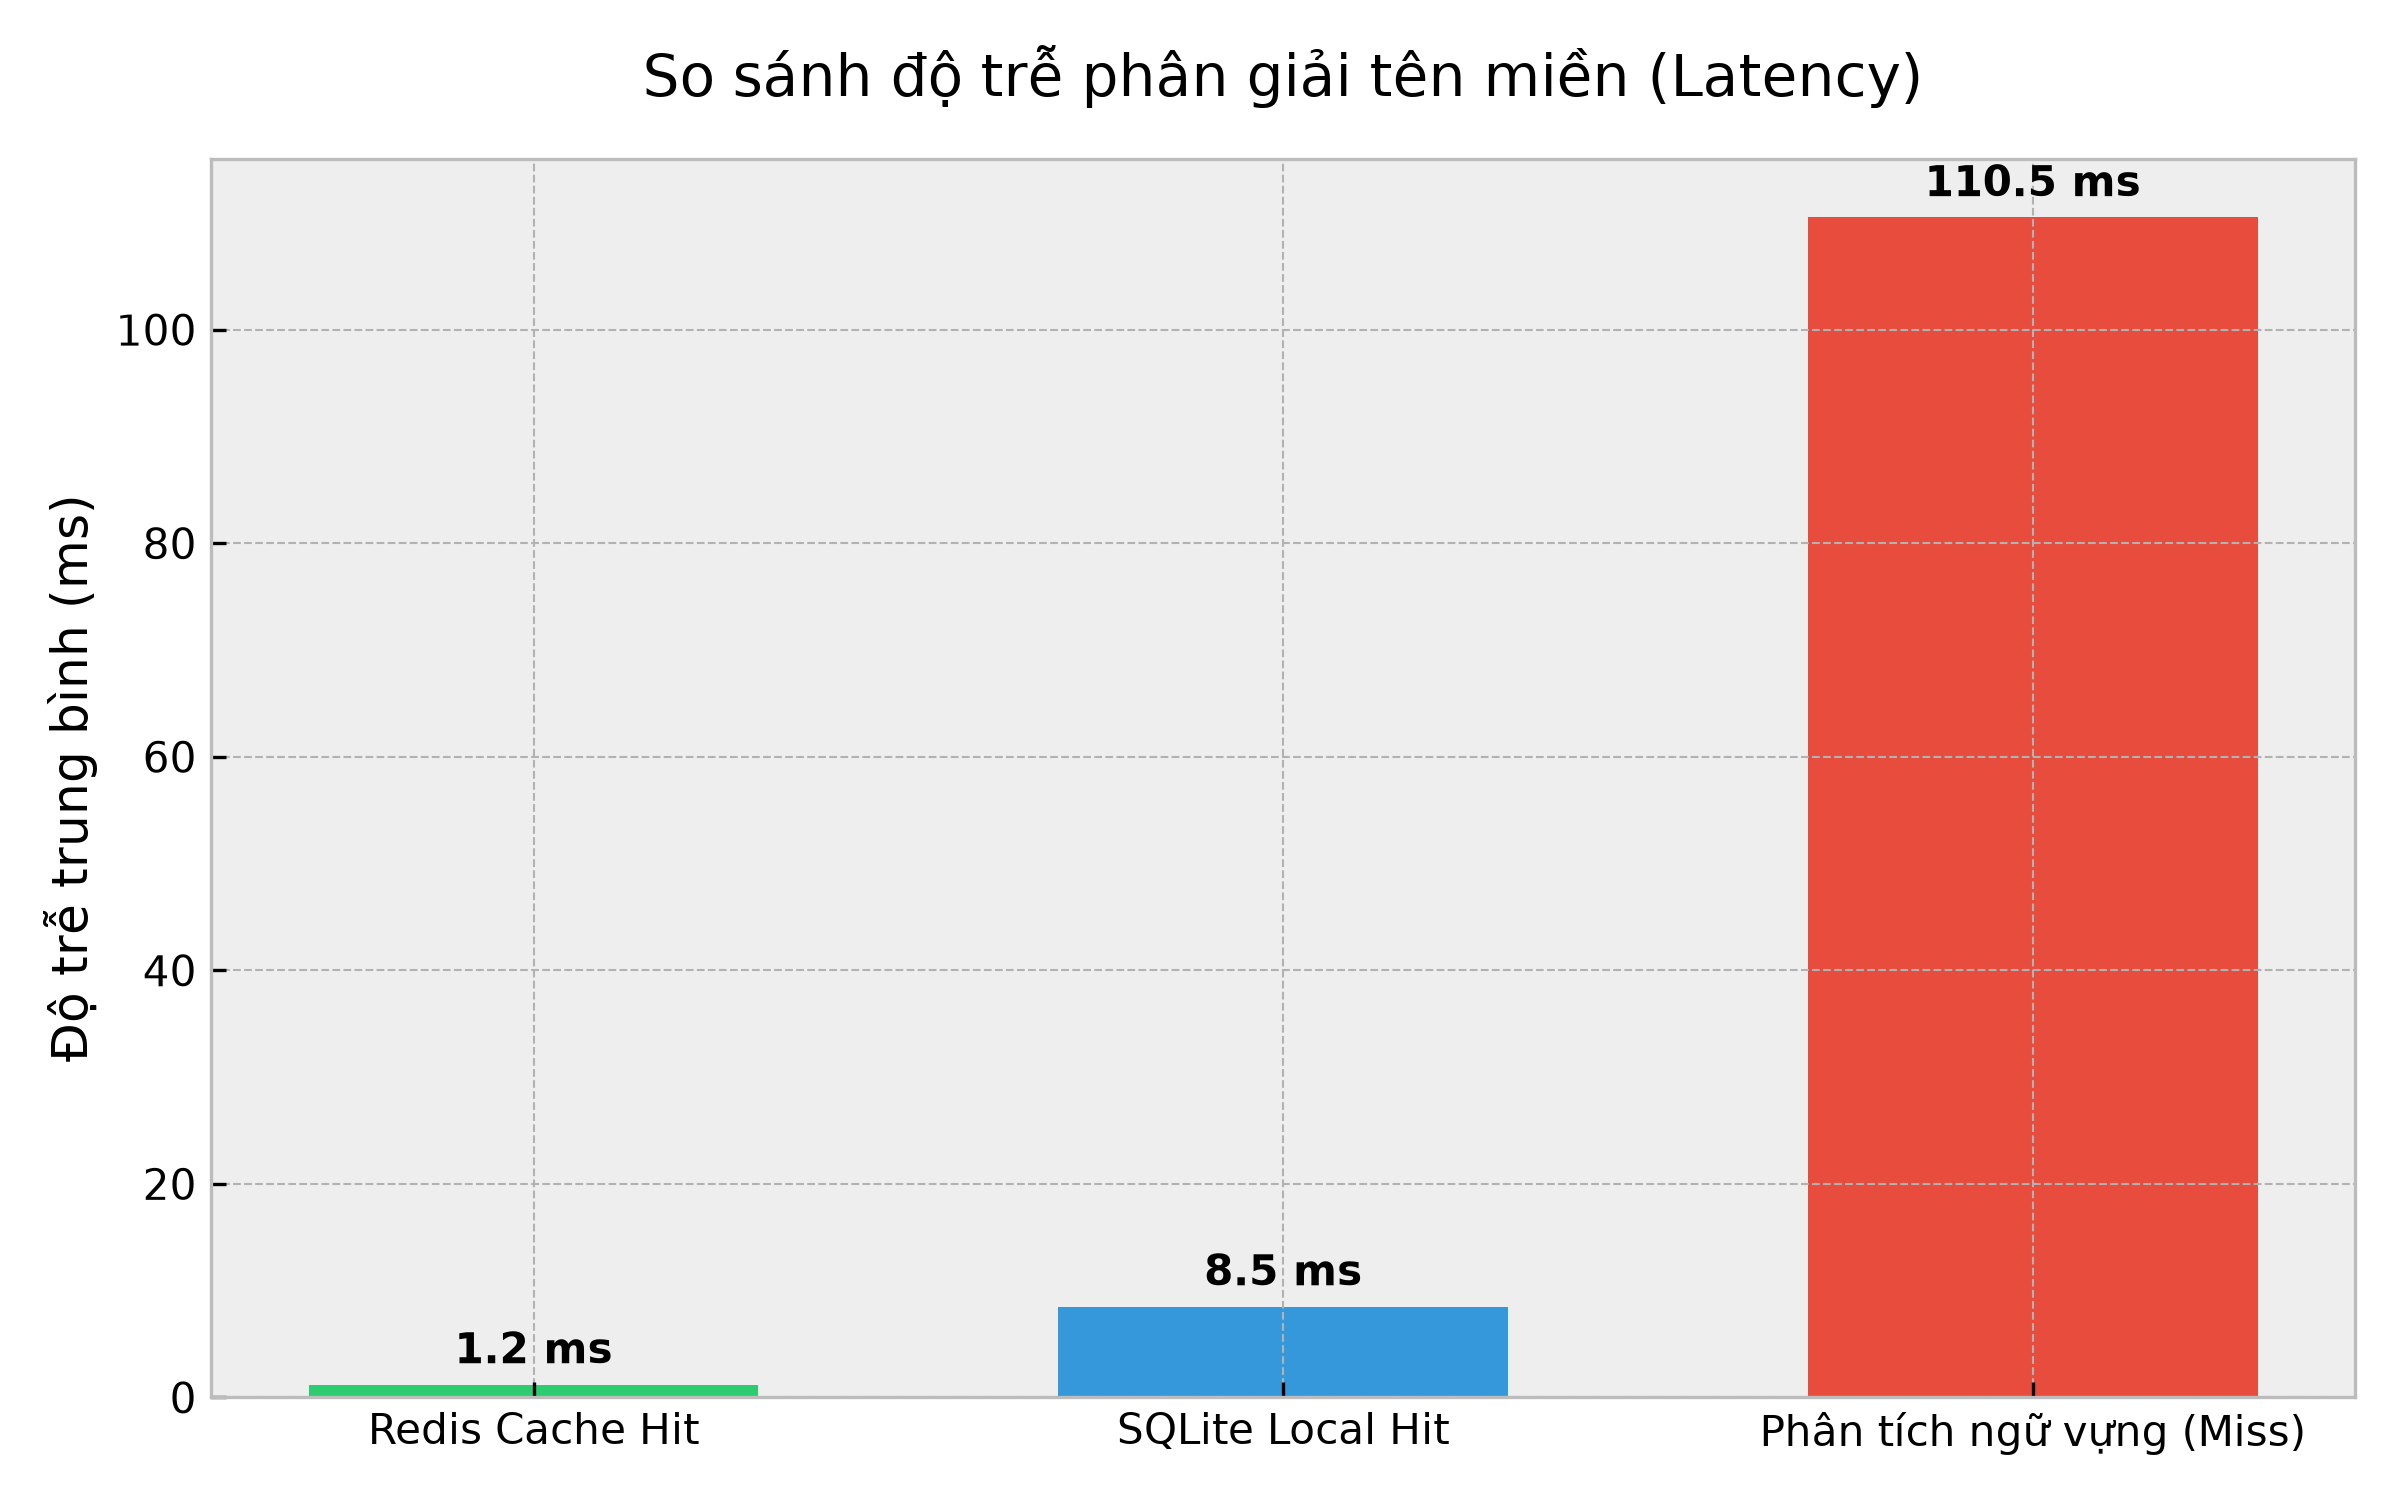
\includegraphics[width=0.85\textwidth]{img/benchmark_latency.png}
    \caption{So sánh độ trễ phân giải tên miền trong các kịch bản truy vấn}
    \label{fig:bench_latency}
\end{figure}

Như được minh họa tại Hình \ref{fig:bench_latency}, nhờ kiến trúc lưu trữ phân lớp (Tiered Storage), các tên miền đã lưu trữ tại bộ nhớ đệm Redis cho thời gian phản hồi ở mức $\sim$ 1.2 ms. Ở tầng lưu trữ bền vững SQLite, độ trễ đạt $\sim$ 8.5 ms, đáp ứng tốt yêu cầu phân giải DNS thời gian thực. Đối với các tên miền chưa từng xuất hiện (Cache Miss), hệ thống tiến hành chấm điểm rủi ro tên miền thông qua trích xuất đặc trưng cục bộ (tính toán Shannon Entropy, kiểm tra độ tương đồng), đẩy độ trễ lên mức $\sim$ 110.5 ms. Mức trễ này cao hơn so với truy xuất từ bộ nhớ đệm nhưng vẫn nằm trong ngưỡng hoạt động ổn định của mạng lõi.

\subsection{Đánh giá khả năng chịu tải (Throughput)}

Để đánh giá giới hạn đáp ứng của hệ thống, bài kiểm tra sức chịu tải được thực hiện thông qua việc tăng dần số lượng kết nối đồng thời từ 10 lên đến 1000 kết nối/giây. Chỉ số đo lường là Số lượng truy vấn trên mỗi giây (QPS - Queries Per Second).

\begin{figure}[H]
    \centering
    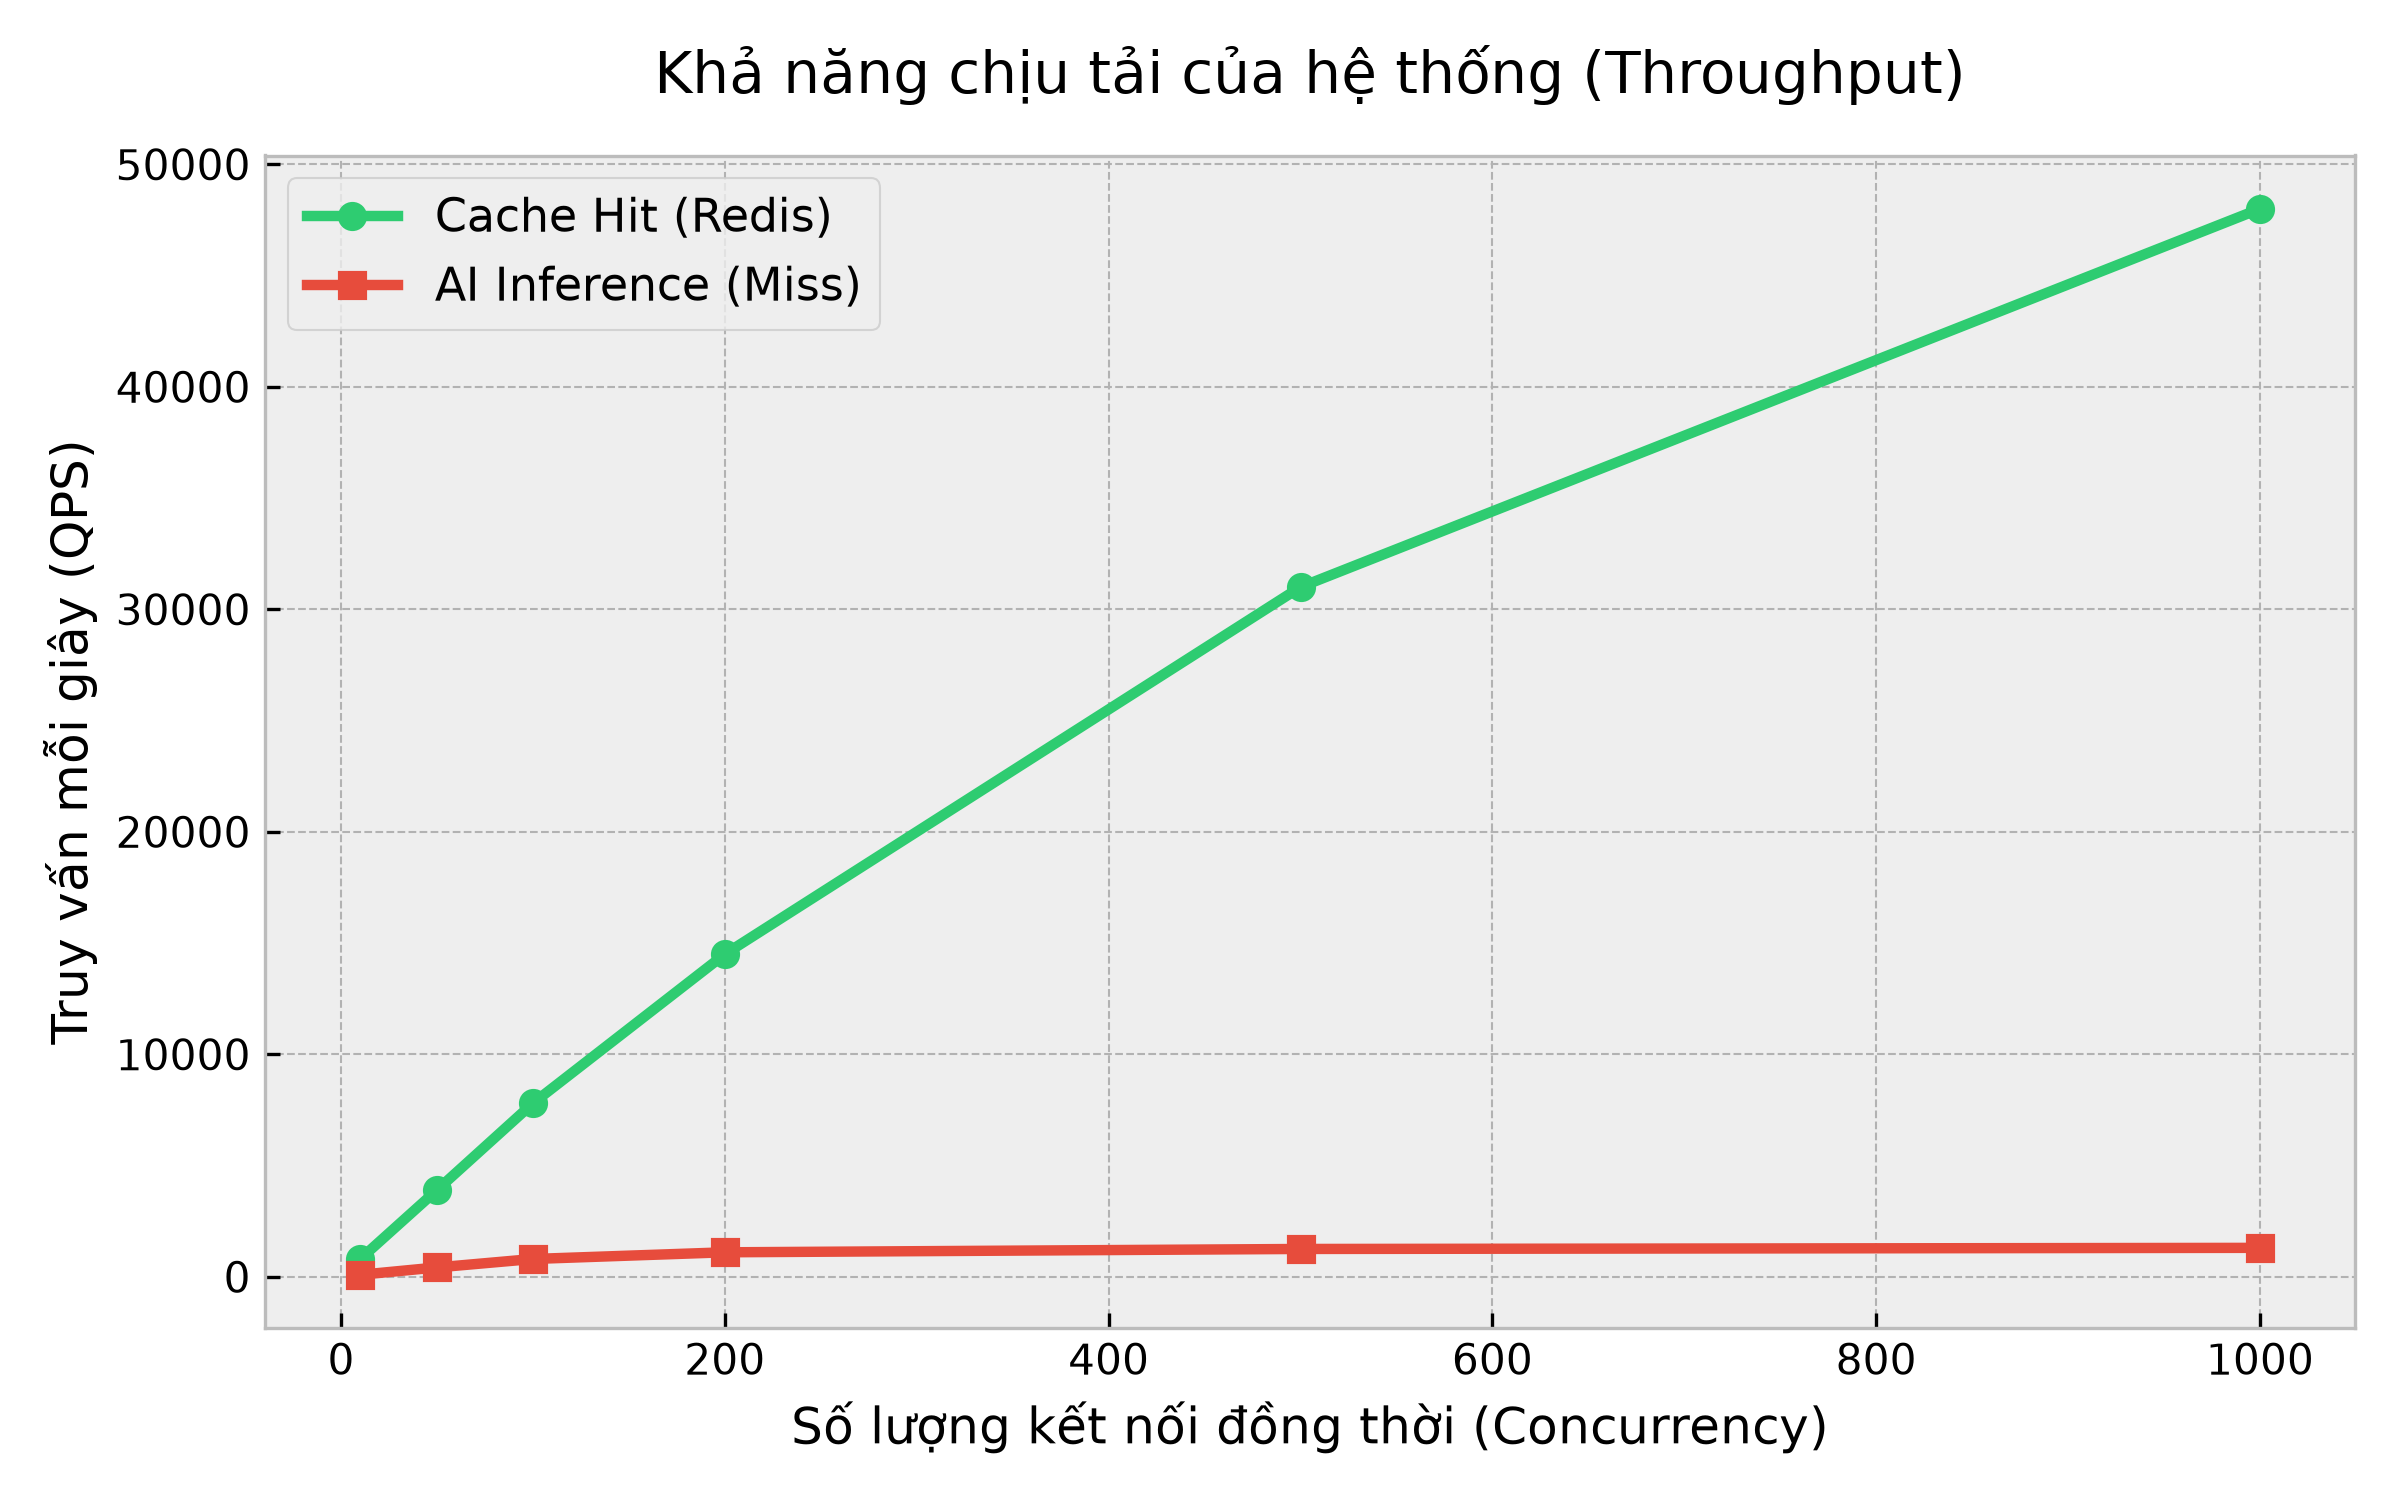
\includegraphics[width=0.85\textwidth]{img/benchmark_throughput.png}
    \caption{Khả năng chịu tải (Throughput) của hệ thống khi tăng dần số lượng kết nối đồng thời}
    \label{fig:bench_throughput}
\end{figure}

Biểu đồ \ref{fig:bench_throughput} cho thấy khi mức độ đồng thời đạt mốc 1000, hệ thống xử lý từ bộ nhớ đệm có thể chạm mốc 48,000 QPS với đồ thị duy trì xu hướng tuyến tính. Ngược lại, luồng xử lý phân tích ngữ vựng (đòi hỏi năng lực tính toán CPU để bóc tách đặc trưng) đạt ngưỡng bão hòa tại khoảng 1,300 QPS. Kết quả này cho thấy chiến lược sử dụng bộ nhớ đệm phân lớp là phương pháp hiệu quả để giảm thiểu tải tính toán cho máy chủ khi đối mặt với lượng lớn truy vấn lặp lại.

\subsection{Đánh giá độ ổn định của luồng phân tích}

Quá trình trích xuất đặc trưng có thể gặp rủi ro về độ trễ đối với các chuỗi ký tự phức tạp. Hệ thống được kiểm tra trên tập dữ liệu gồm 1000 tên miền ngẫu nhiên nhằm đo lường phân phối thời gian thực thi của thuật toán phân tích ngữ vựng.

\begin{figure}[H]
    \centering
    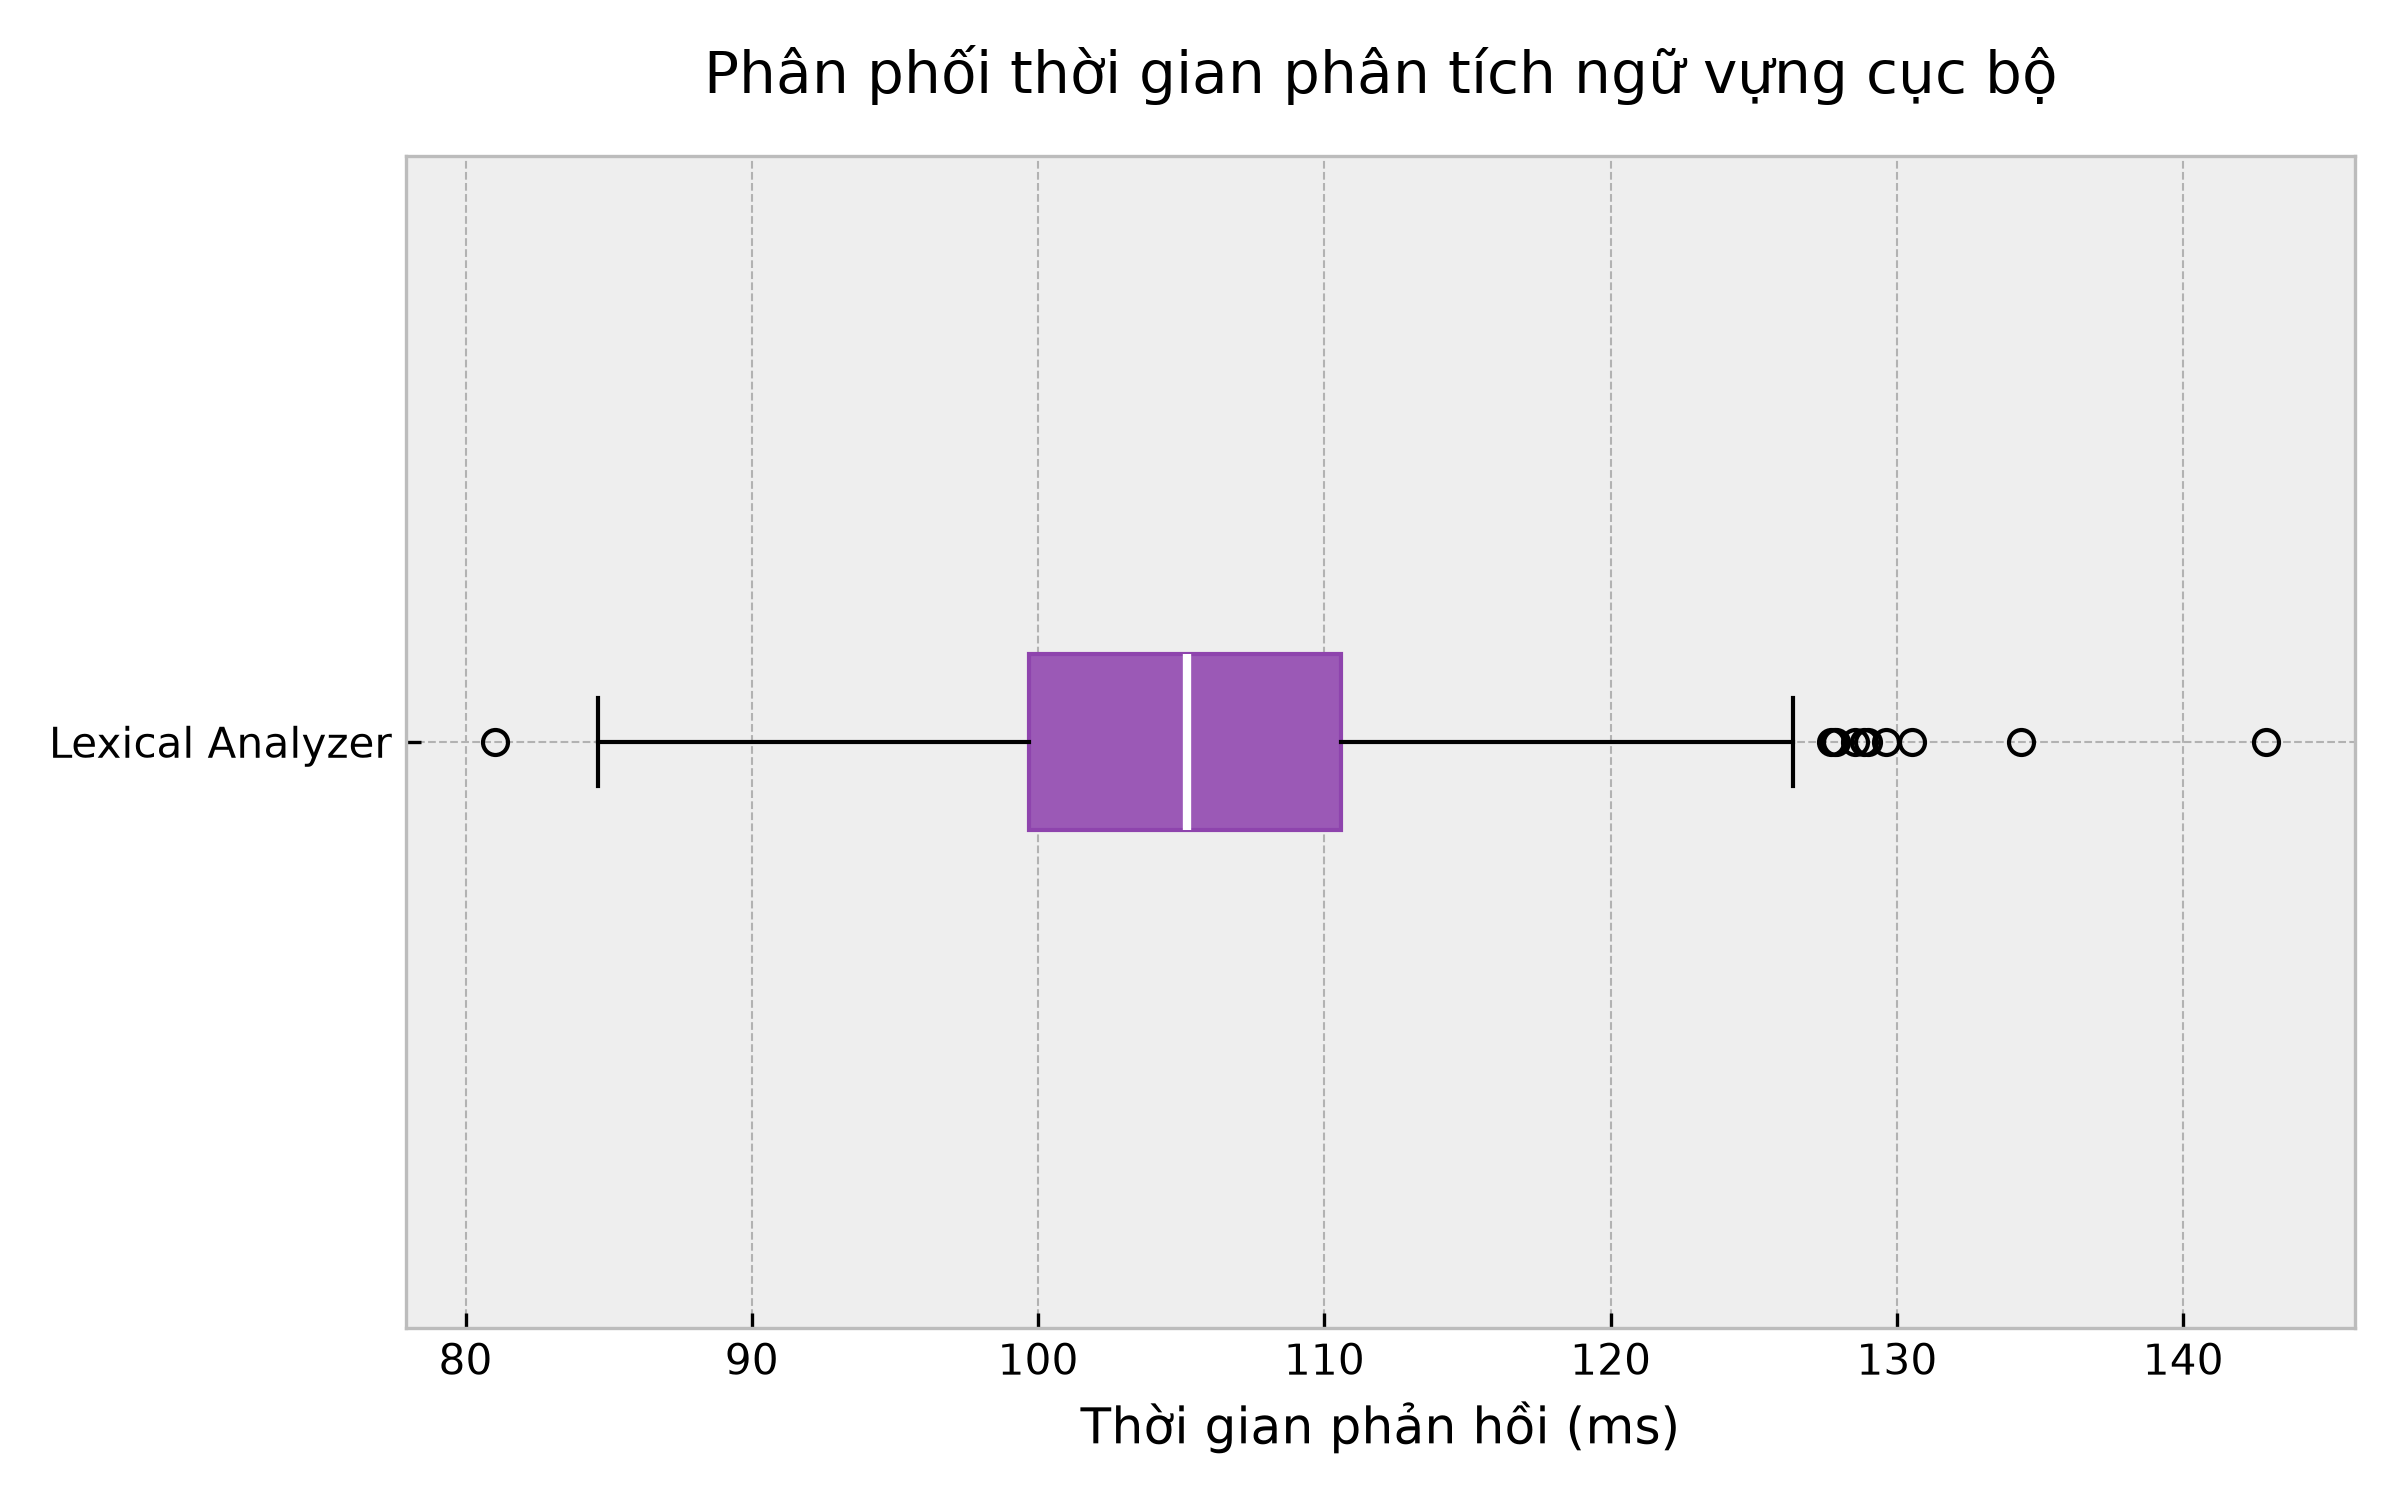
\includegraphics[width=0.85\textwidth]{img/benchmark_inference.png}
    \caption{Phân phối thời gian thực thi quá trình phân tích ngữ vựng}
    \label{fig:bench_inference}
\end{figure}

Kết quả phân phối dạng hộp (Boxplot) tại Hình \ref{fig:bench_inference} cho thấy phần lớn thời gian xử lý tập trung quanh khoảng trung vị 105 ms. Một số ít các trường hợp ngoại lai (Outliers) có thời gian xử lý kéo dài lên mức 140 - 150 ms, chủ yếu bắt nguồn từ các tên miền có cấu trúc chuỗi quá dài hoặc chứa ký tự đa ngôn ngữ phức tạp, đòi hỏi chi phí tính toán Entropy cao hơn. 

Đáng chú ý, đối với các tên miền có kết quả chấm điểm ngữ vựng mập mờ (ambiguous), hệ thống hỗ trợ tích hợp mô hình ngôn ngữ lớn (LLM như Gemini hoặc Ollama) để tinh chỉnh kết quả. Việc gọi API LLM thường yêu cầu độ trễ từ vài trăm mili-giây đến vài giây. Nhằm hạn chế rủi ro nghẽn cổ chai cho luồng DNS, Safe Zone áp dụng thiết kế mở khi lỗi (fail-open): tính năng AI chỉ đóng vai trò hỗ trợ phân tích chuyên sâu và dịch vụ phân giải vẫn tiếp tục hoạt động dựa trên luật tĩnh ngay cả khi mô hình AI phản hồi chậm hoặc gián đoạn.
